\subsection{Glyph: \glyph{Uncertain process}}
\label{sec:uncertain}

Uncertain processes are processes that may not exist. A single \glyph{uncertain process} can represent any number of actual processes.

\begin{glyphDescription}

\glyphSboTerm
SBO:0000396 ! uncertain process

\corr{\glyphOrigin
One or several \glyph{consumption} arcs (\sect{consumption}) or one or several \glyph{production} arcs (\sect{production}).
}{
\glyphIncoming
One ore more \glyph{consumption} arcs (\sect{consumption})\footnote{Zero \glyph{consumption arcs} are allowed in the case of a reversible process.}, zero or more \glyph{modulation} arcs (\sect{modulations}).
}

\corr{\glyphTarget
One or several \glyph{production} arcs (\sect{production}).
}{
\glyphOutgoing
One or more \glyph{production} arcs (\sect{production}).
}

\glyphContainer
A \glyph{process} is represented by a square shape containing a question mark.
The shape is linked to two ports, that are small arcs attached to the centres of opposite sides of the shape, as shown in \fig{uncertain}.
The incoming \glyph{consumption} (\sect{consumption}) and outgoing \glyph{production} (\sect{production}) arcs are linked to the extremities of those ports.

The \glyph{modulation arcs} (\sect{modulations}) point to the other two sides of the shape.

\glyphLabel
\corr{An \glyph{uncertain process} is not identified by any label}{None}.

\glyphAux
\corr{An \glyph{uncertain process} does not carry any auxiliary items}{None}.

\end{glyphDescription}

\begin{figure}[H]
  \centering
  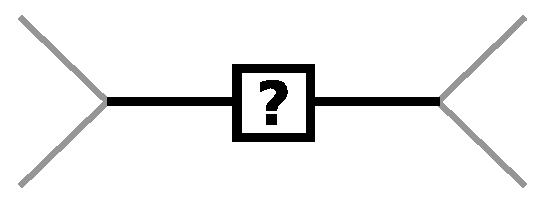
\includegraphics{images/uncertain}
  \caption{The \PD glyph for an \glyph{uncertain process}.}
  \label{fig:uncertain}
\end{figure}
